%!TEX root=../tax-democracy-held.tex

\begin{landscape}
 \begin{table}[htbp]
	\begin{center}
	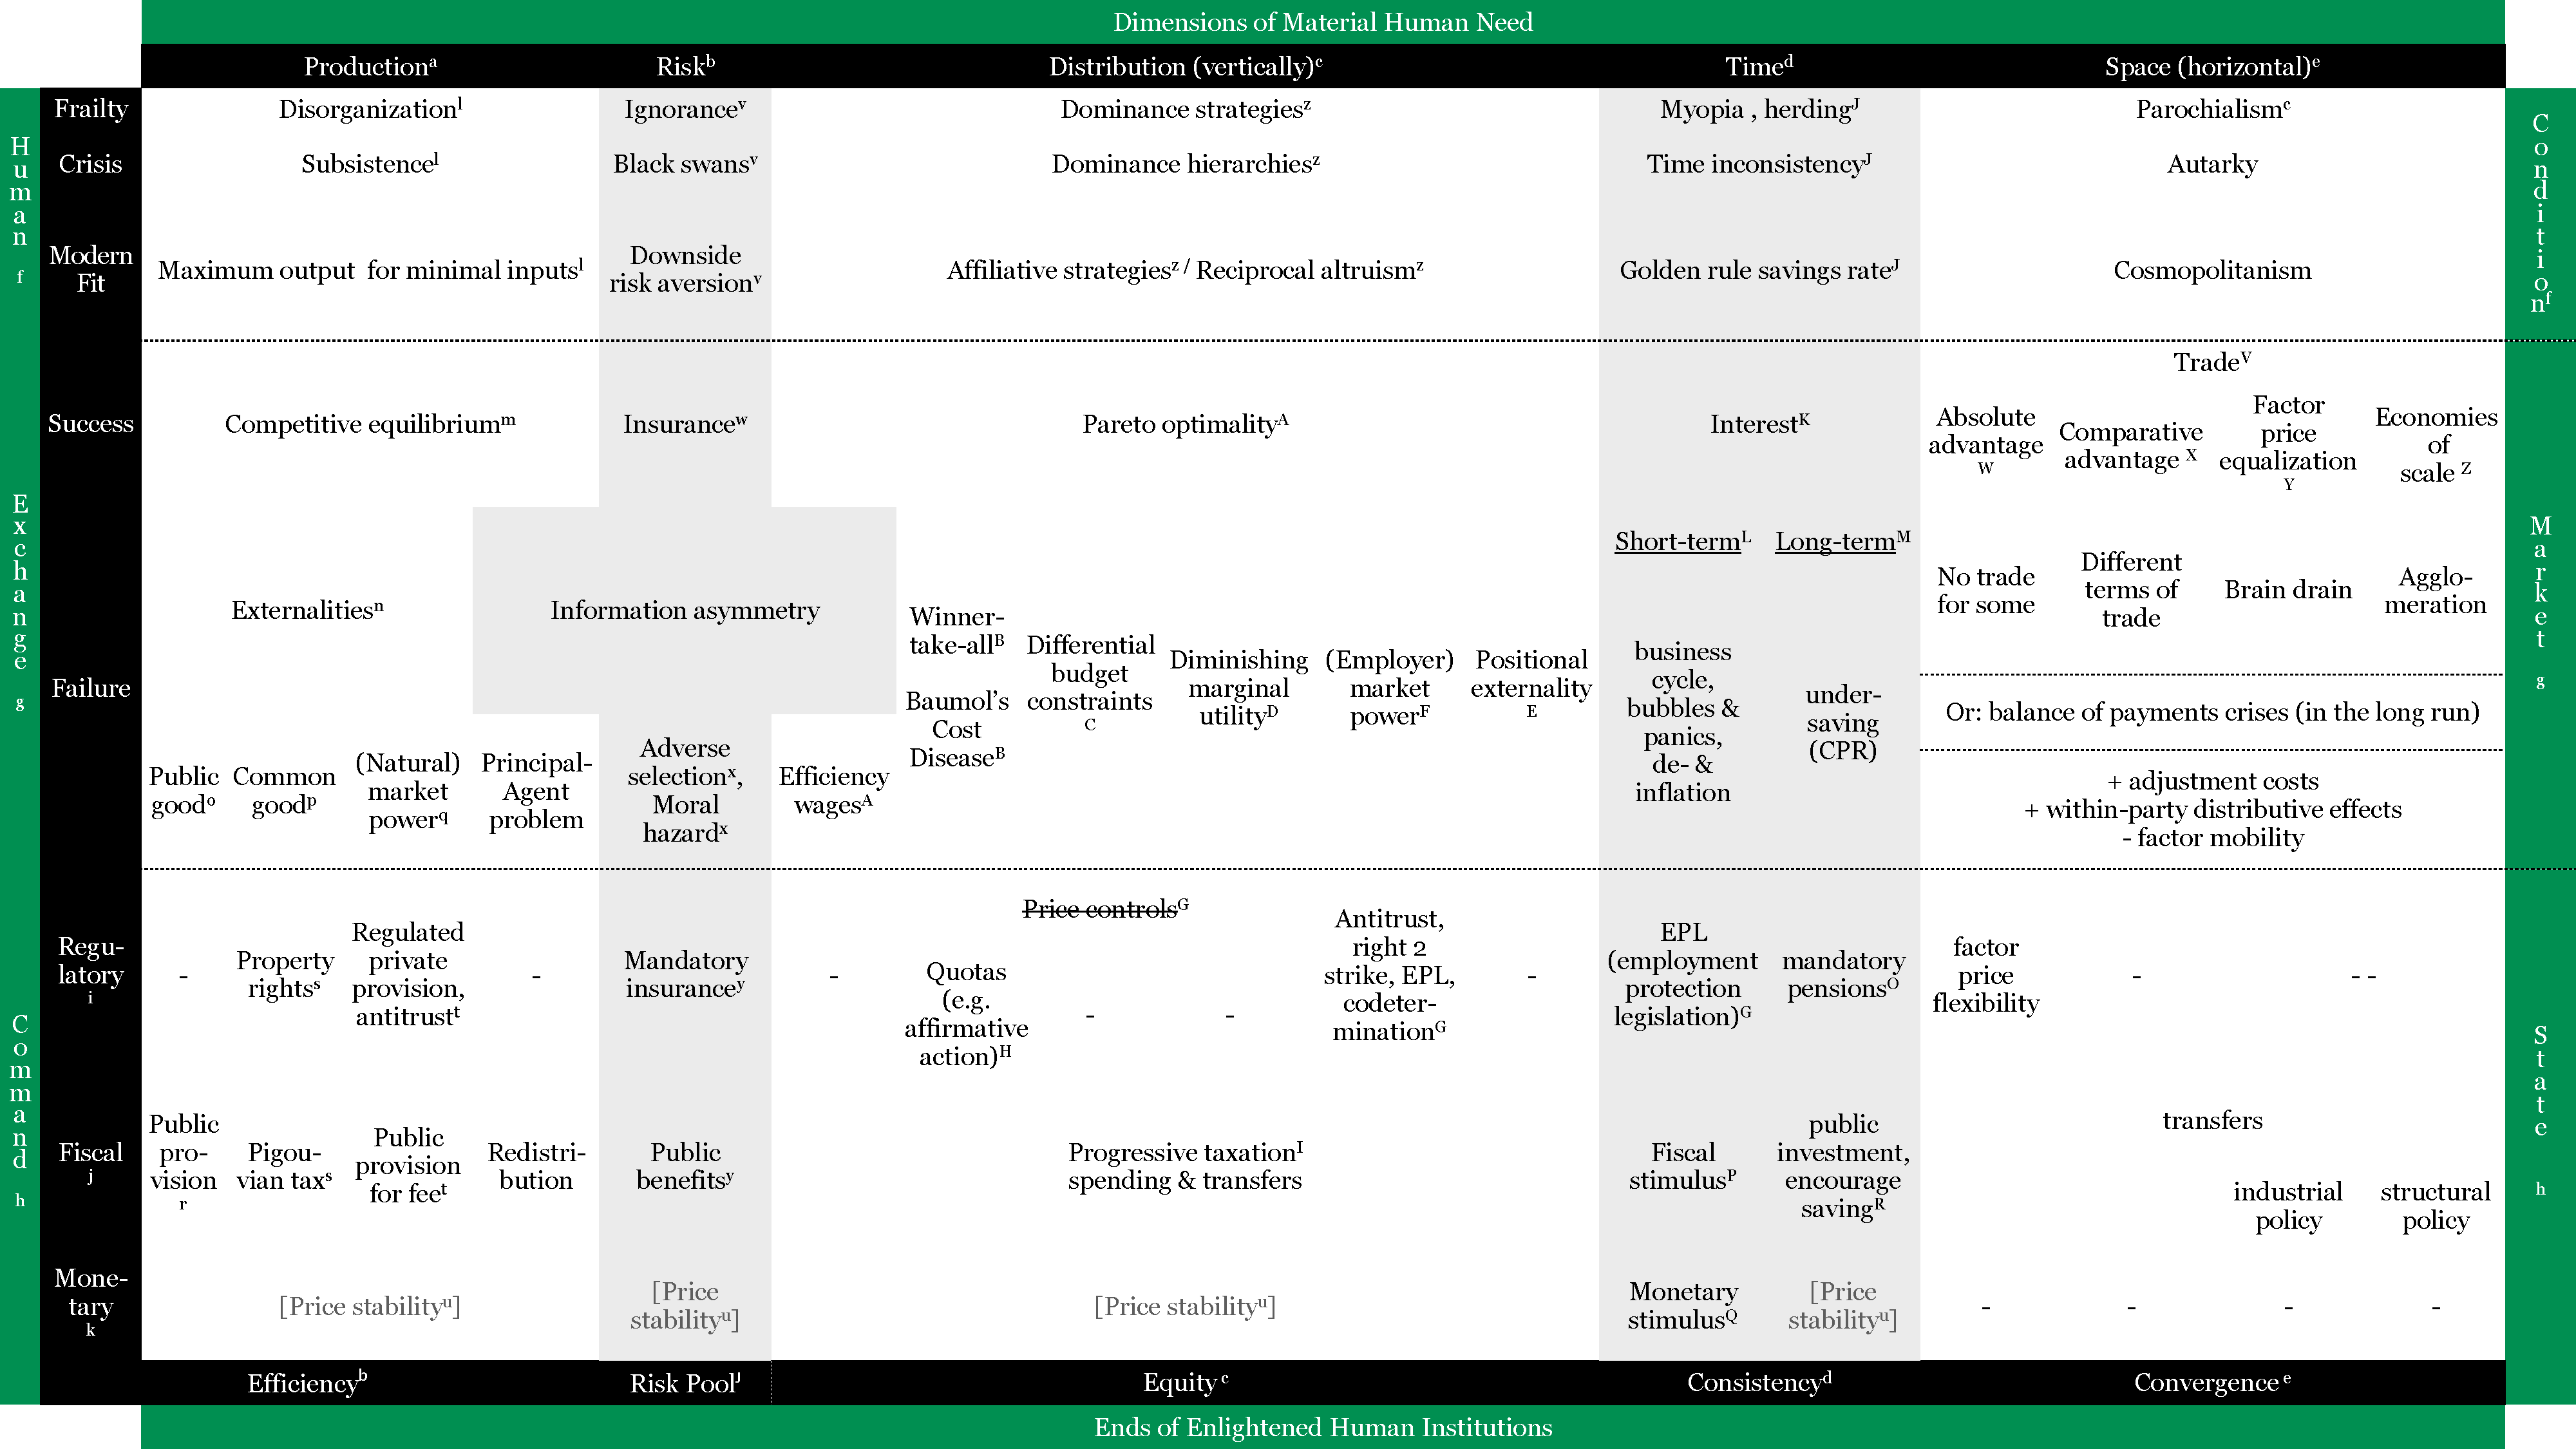
\includegraphics[width=1\linewidth]{ends-mixed-economy}
	\caption{Ends of the Mixed Economy \label{tab:ends-mixed-economy}}
\end{center}
\newpage
\end{table}
\end{landscape}\footnote{
Read the table from top to bottom, then from left to right.
For every material dimension (column), I first present the human condition (first three rows), then market (exchange) solutions and problems (next two rows) and then present corresponding state (command) responses by fiscal, regulatory and monetary means (bottom three rows)
The headings of following sections correspond to the column headings.

		\emph{a}: \nameref{sec:production} on page \pageref{sec:production},
		\emph{b}: \nameref{sec:risk} on page \pageref{sec:risk},
		\emph{c}: \nameref{sec:distribution} on page \pageref{sec:distribution},
		\emph{d}: \nameref{sec:time} on page \pageref{sec:time},
		\emph{e}: \nameref{sec:space} on page \pageref{sec:space},
		\emph{f}: \nameref{sec:human-nature} on page \pageref{sec:human-nature},
		\emph{g}: \nameref{sec:exchange} on page \pageref{sec:exchange},
		\emph{h}: \nameref{sec:command} on page \pageref{sec:command},
		\emph{i}: \nameref{sec:regulatory} on page \pageref{sec:regulatory},
		\emph{j}: \nameref{sec:fiscal} on page \pageref{sec:fiscal},
		\emph{k}: \nameref{sec:monetary} on page \pageref{sec:monetary},
		\emph{l}: \nameref{sec:human-nature-of-production} on page \pageref{sec:human-nature-of-production},
		\emph{m}: \nameref{sec:market-solutions-production} on page \pageref{sec:market-solutions-production},
		\emph{n}: \nameref{sec:market-failures} on page \pageref{sec:market-failures} and see \autoref{tab:types-of-goods},
		\emph{o}: \nameref{sec:public-good} on page \pageref{sec:public-good},
		\emph{p}: \nameref{sec:common-good} on page \pageref{sec:common-good},
		\emph{q}: \nameref{sec:natural-monopoly} on page \pageref{sec:natural-monopoly},
		\emph{r}: \nameref{sec:public-good-response} on page \pageref{sec:public-good-response},
		\emph{s}: \nameref{sec:common-good-response} on page \pageref{sec:common-good-response},
		\emph{t}: \nameref{sec:natural-monopoly-response} on page \pageref{sec:natural-monopoly-response},
		\emph{u}: \nameref{sec:price-stability} on page \pageref{sec:price-stability},
		\emph{v}: \nameref{sec:human-nature-of-risk} on page \pageref{sec:human-nature-of-risk},
		\emph{w}: \nameref{sec:insurance} on page \pageref{sec:insurance},
		\emph{x}: \nameref{sec:asymmetric-information} on page \pageref{sec:asymmetric-information},
		\emph{y}: \nameref{sec:state-insurance} on page \pageref{sec:state-insurance},
		\emph{z}: \nameref{sec:human-nature-of-inequality} on page \pageref{sec:human-nature-of-inequality},
		\emph{A}: \nameref{sec:market-equity} on page \pageref{sec:market-equity},
		\emph{AA}: \nameref{sec:efficiency-wages} on page \pageref{sec:efficiency-wages},
		\emph{B}: \nameref{sec:winner-take-all} on page \pageref{sec:winner-take-all},
		\emph{C}: \nameref{sec:different-budget-constraints} on page \pageref{sec:different-budget-constraints},
		\emph{D}: \nameref{sec:diminishing-marginal-utility} on page \pageref{sec:diminishing-marginal-utility},
		\emph{F}: \nameref{sec:monopsony-employers} on page \pageref{sec:monopsony-employers},
		\emph{E}: \nameref{sec:positional-race} on page \pageref{sec:positional-race},
		\emph{G}: \nameref{sec:price-controls} on page \pageref{sec:price-controls},
		\emph{H}: \nameref{sec:affirmative-action} on page \pageref{sec:affirmative-action},
		\emph{I}: \nameref{sec:fiscal-redistribution} on page \pageref{sec:fiscal-redistribution},
		\emph{J}: \nameref{sec:time} on page \pageref{sec:time},
		\emph{K}: \nameref{sec:interest} on page \pageref{sec:interest},
		\emph{L}: \nameref{sec:short-term-inconsistency} on page \pageref{sec:short-term-inconsistency},
		\emph{M}: \nameref{sec:long-term-inconsistency} on page \pageref{sec:long-term-inconsistency},
		\emph{O}: \nameref{sec:government-saves} on page \pageref{sec:government-saves},
		\emph{P}: \nameref{sec:fiscal-stimulus} on page \pageref{sec:fiscal-stimulus},
		\emph{Q}: \nameref{sec:monetary-stimulus} on page \pageref{sec:monetary-stimulus},
		\emph{R}: \nameref{sec:government-saves} on page \pageref{sec:government-saves},
		\emph{S}: \nameref{sec:government-saves} on page \pageref{sec:government-saves},
		\emph{V}: \nameref{sec:trade} on page \pageref{sec:trade},
		\emph{W}: \nameref{itm:absolute-advantage} on page \pageref{itm:absolute-advantage},
		\emph{X}: \nameref{itm:comparative-advantage} on page \pageref{itm:comparative-advantage},
		\emph{Y}: \nameref{itm:FPE} on page \pageref{itm:FPE},
		\emph{Z}: \nameref{itm:NTT} on page \pageref{itm:NTT}.}

% \begin{table}[htbp]
	%	\centering
	%	\rotatebox{90}{
	%	\begin{minipage}{\textheight}
	%	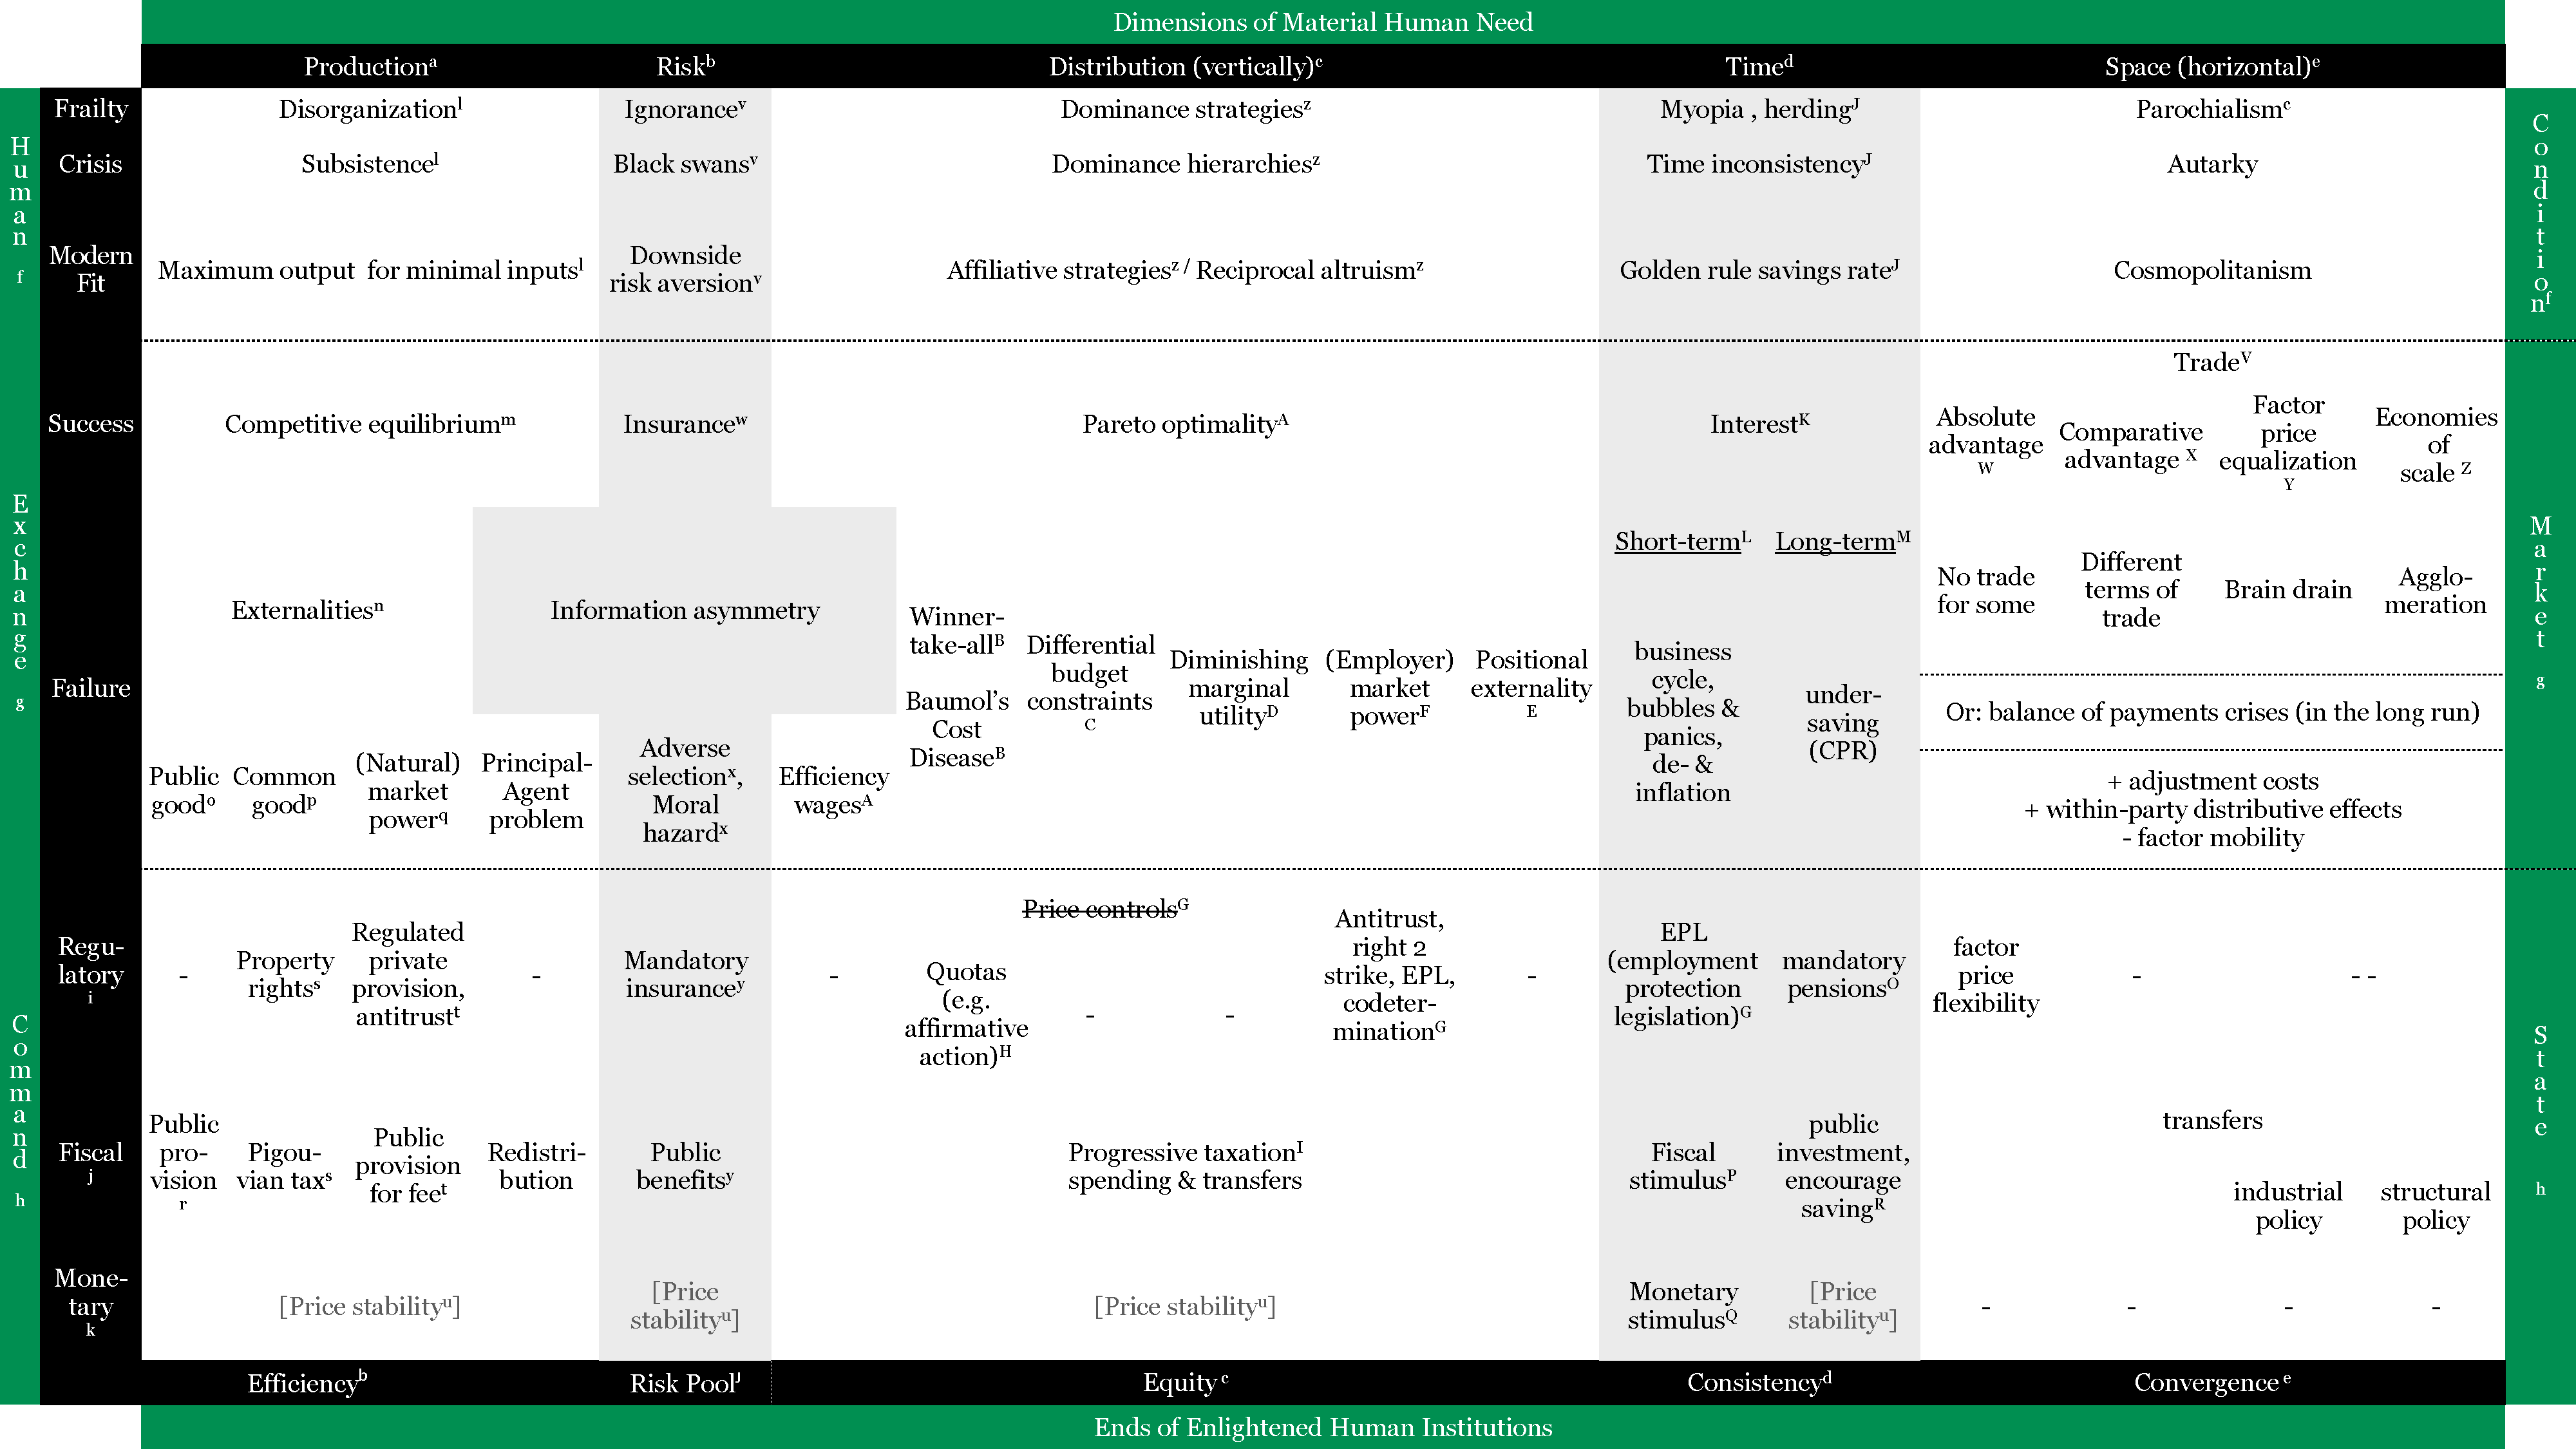
\includegraphics[width=1\linewidth]{ends-mixed-economy}
	%	\caption{Ends of the Mixed Economy}
	%	\label{tab:ends-mixed-economy}
	%	\end{minipage}
	%	}
%\end{table}

%\includepdf[landscape=true , fitpaper=true, frame=true ]{ends-mixed-econ}
	%if you want to go back and use this, you have to enable pdfpages package